% !TEX root = main.tex

\newpage
\section{Results}

%%%%%%%%%%%%%%%%%%%%%%%%%%%%%%%%%%%%%%%%%%%%%%%%%%%%%%%%%%%%%%%%%%
\subsection{Examples}

We first demonstrate a qualitative example of this approach applied to a 2D wave equation with a radially symmetric initial condition.
\FloatBarrier
%\begin{center}
\begin{figure}[H]
    \begin{tabular}{cc}
        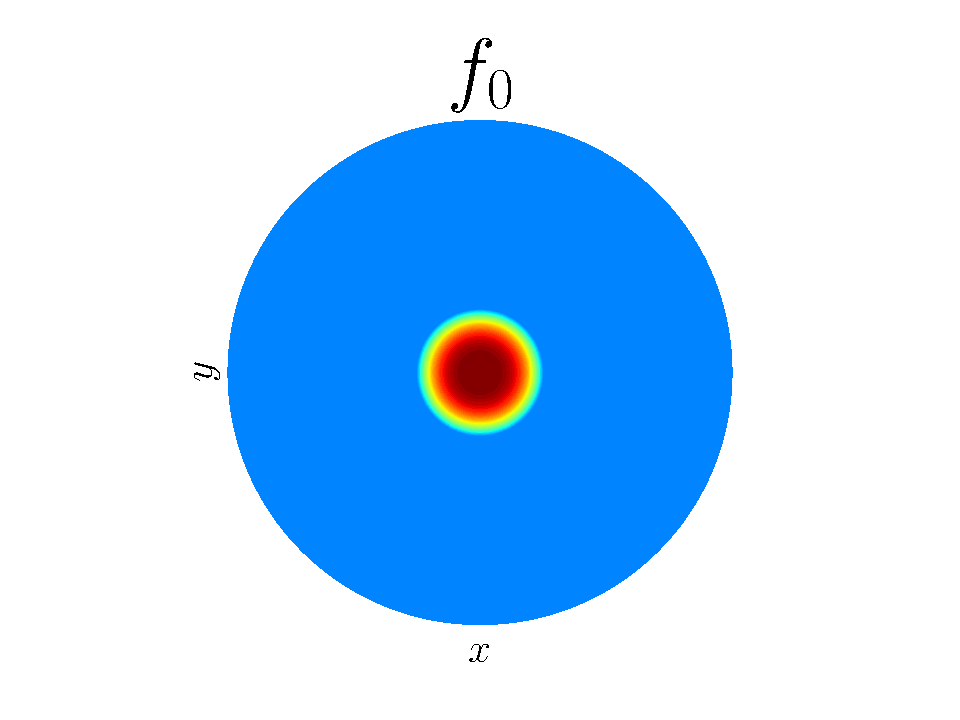
\includegraphics[height=5cm]{figures/Physical_Initial.pdf} & 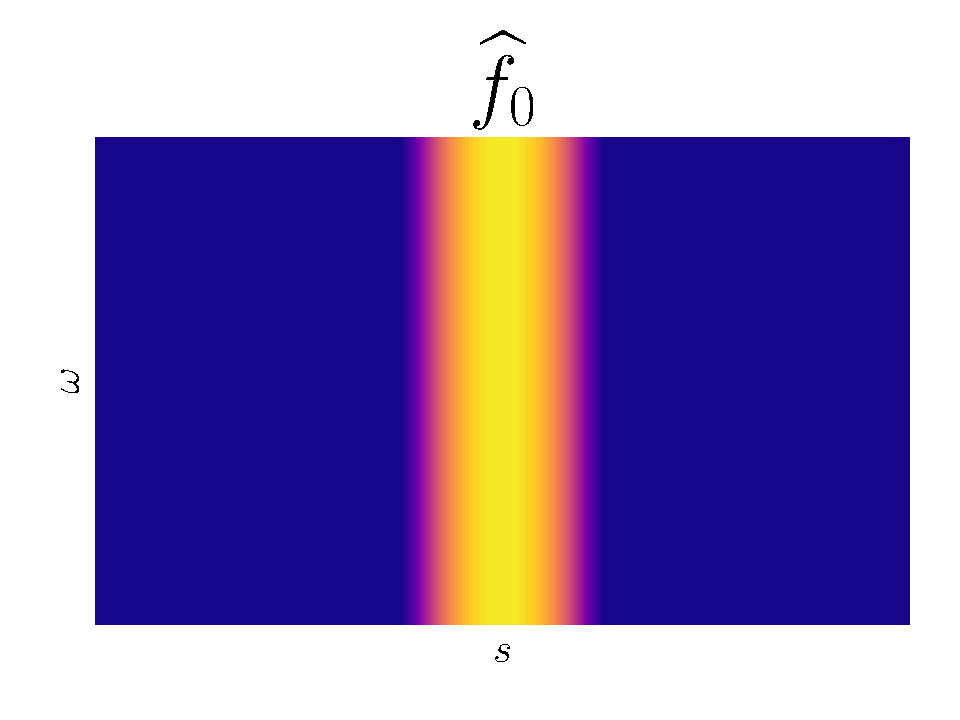
\includegraphics[height=5cm]{figures/Radon_Initial.pdf} \\ 
        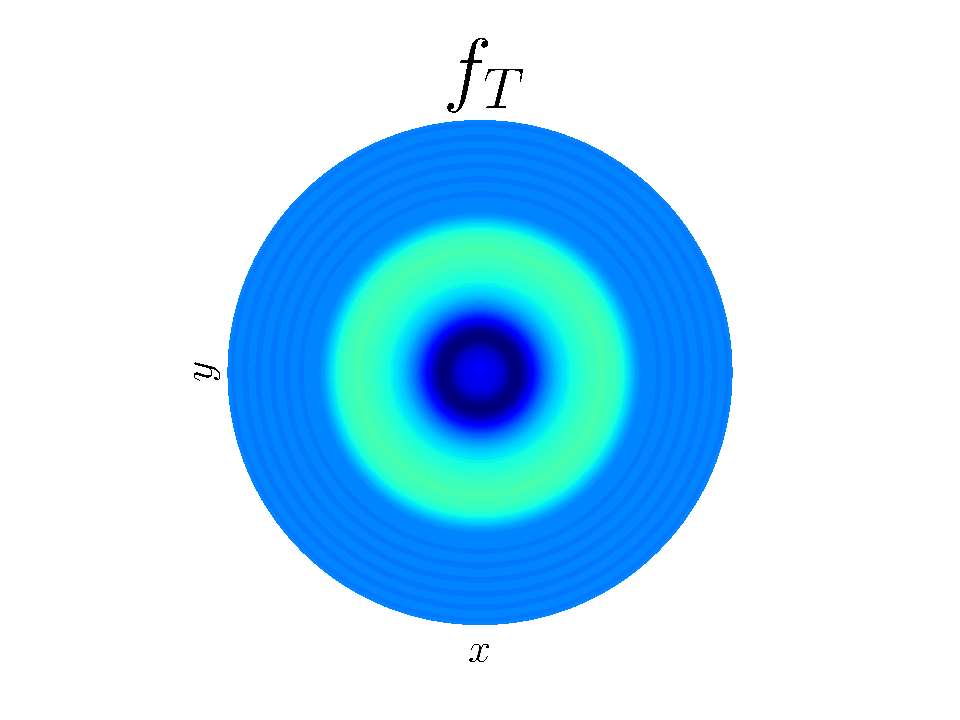
\includegraphics[height=5cm]{figures/Physical_Final.pdf} & 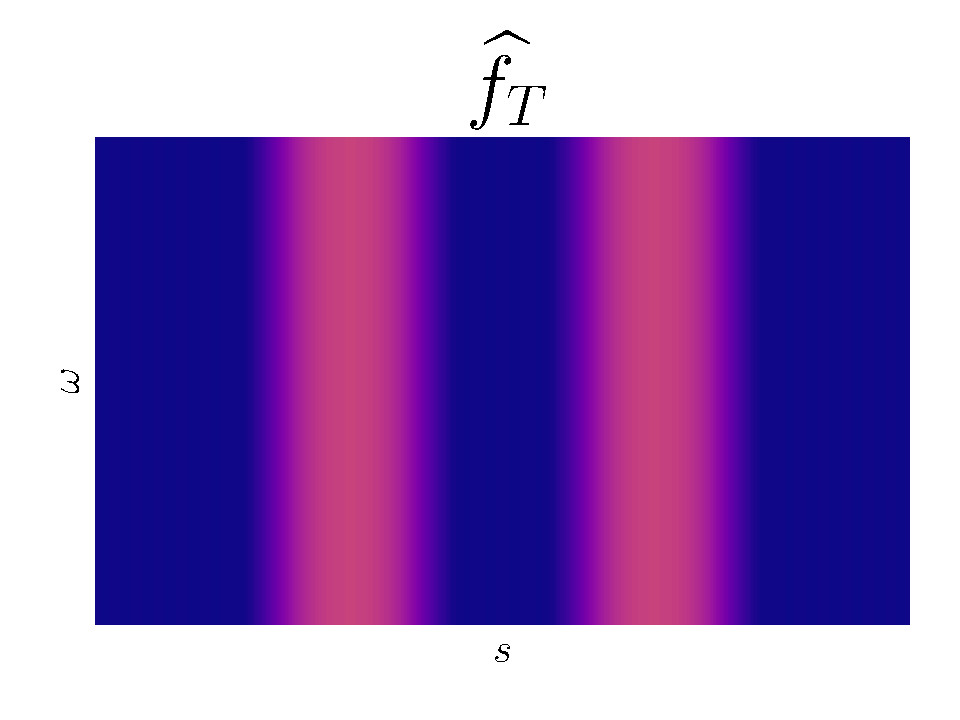
\includegraphics[height=5cm]{figures/Radon_Final.pdf}
    \end{tabular}
    \caption{Wave equation initial conditions (top) and final solution (bottom) \\ in physical (left) and Radon space (right)}
\end{figure}
%\end{center}
\FloatBarrier
In the above figures, we can observe the effect of Radial symmetry on our method. In particular, each sample of radon space is identical, as the transform is independent of the angle $\omega$. Moreover, the inversion process is much simpler, as the Radon transform matrix $\mat{R}$ is initially well conditioned and can be simply inverted.

\newpage
We can repeat this process for the radially symmetric $P_1$ equations. We use the standard initial condition, the following approximate to a Dirac delta function with $\alpha = 0.03$:
\begin{align*}
    q_0(x, y) = \frac{1}{4\pi\alpha^2}e^{\frac{ -(x^2 + y^2) }{4\alpha^2} }
\end{align*}
\FloatBarrier
\begin{center}
\begin{figure}[H]
    \begin{tabular}{c|c}
        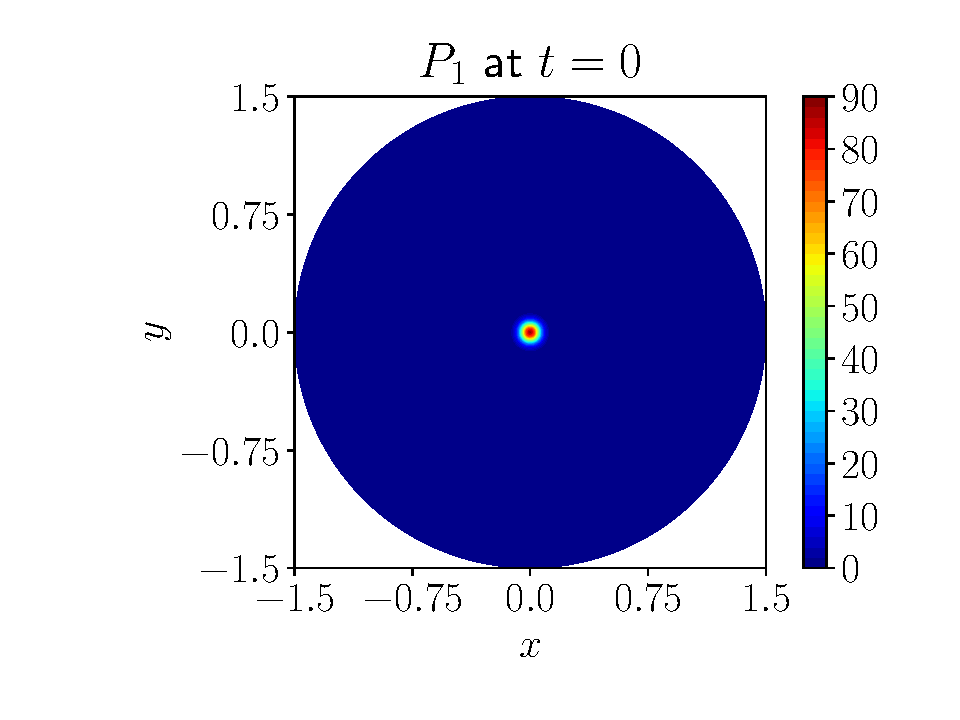
\includegraphics[height=5cm]{figures/physical_inital_p1.pdf} & 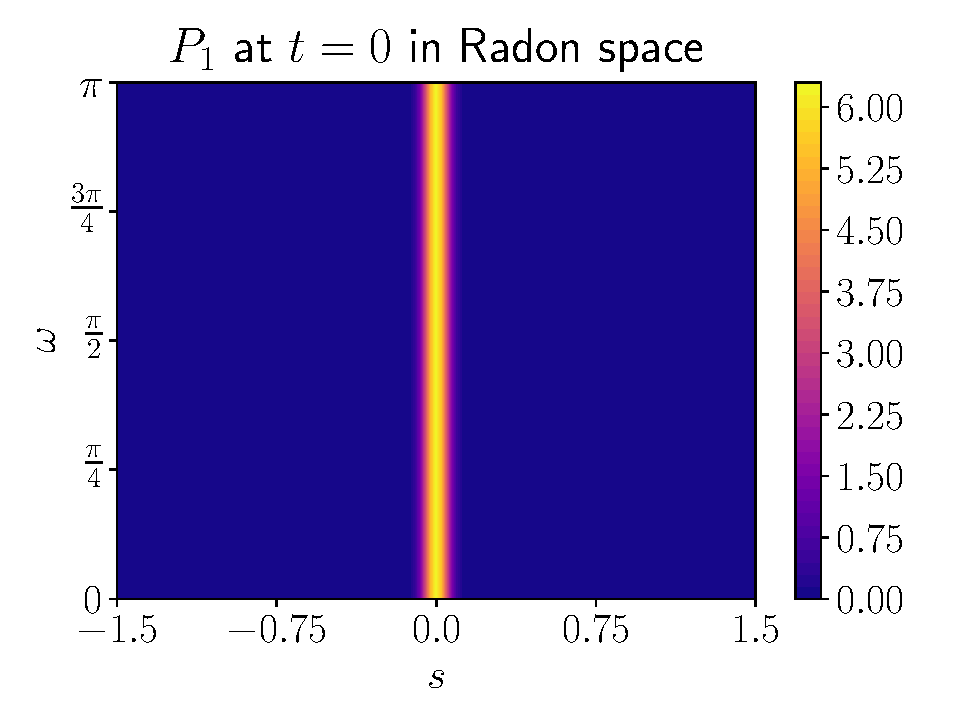
\includegraphics[height=5cm]{figures/radon_inital_p1.pdf} \\ \hline
        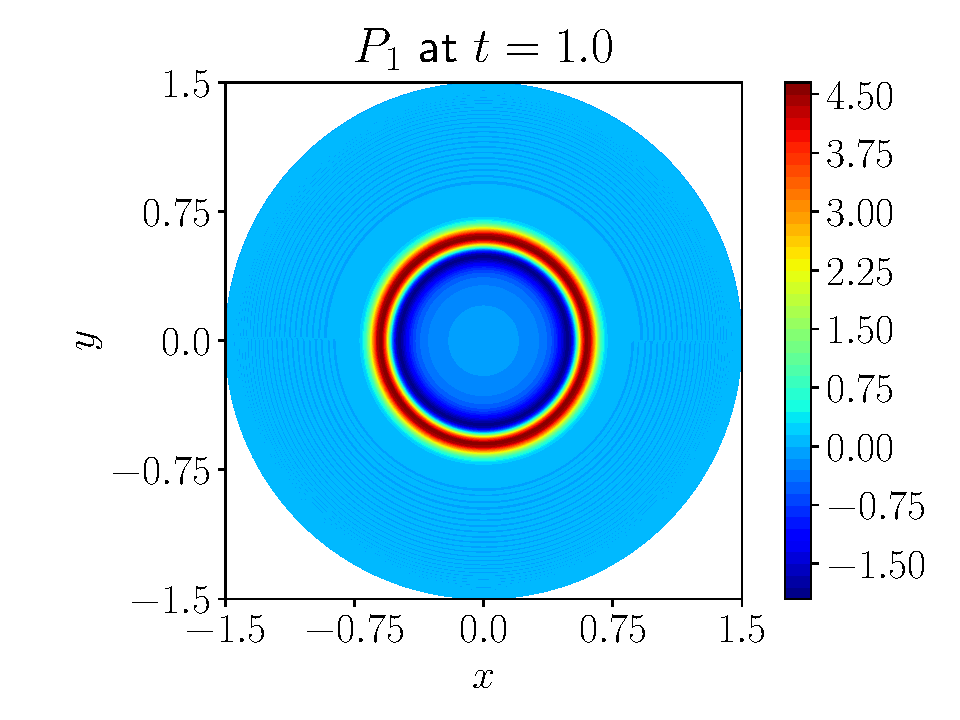
\includegraphics[height=5cm]{figures/physical_final_p1.pdf} & 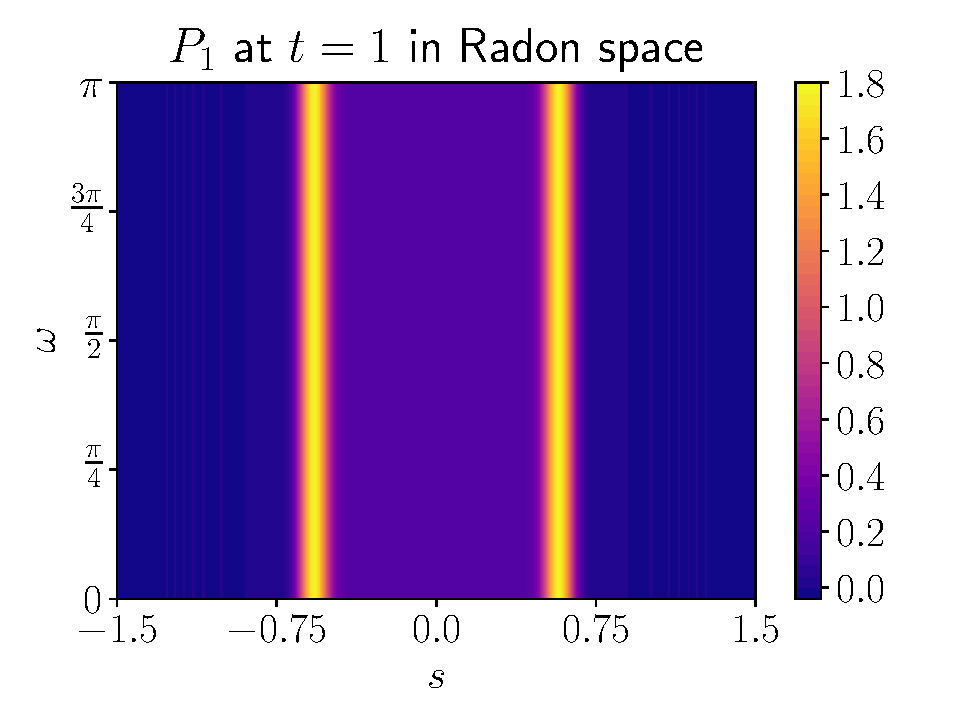
\includegraphics[height=5cm]{figures/radon_final_p1.pdf}
    \end{tabular}
    \caption{$P_1$ initial conditions (top) and final solution (bottom) \\ in physical (left) and Radon space (right)}
\end{figure}
\end{center}
\FloatBarrier
Because the $P_N$ equations themselves are only approximations of radiative transfer, we increase $N$ and compare our results to those in\cite{Shin:6}, as we see on the following page.

\newpage
\FloatBarrier
\begin{center}
\begin{tabular}{c|c}                    
    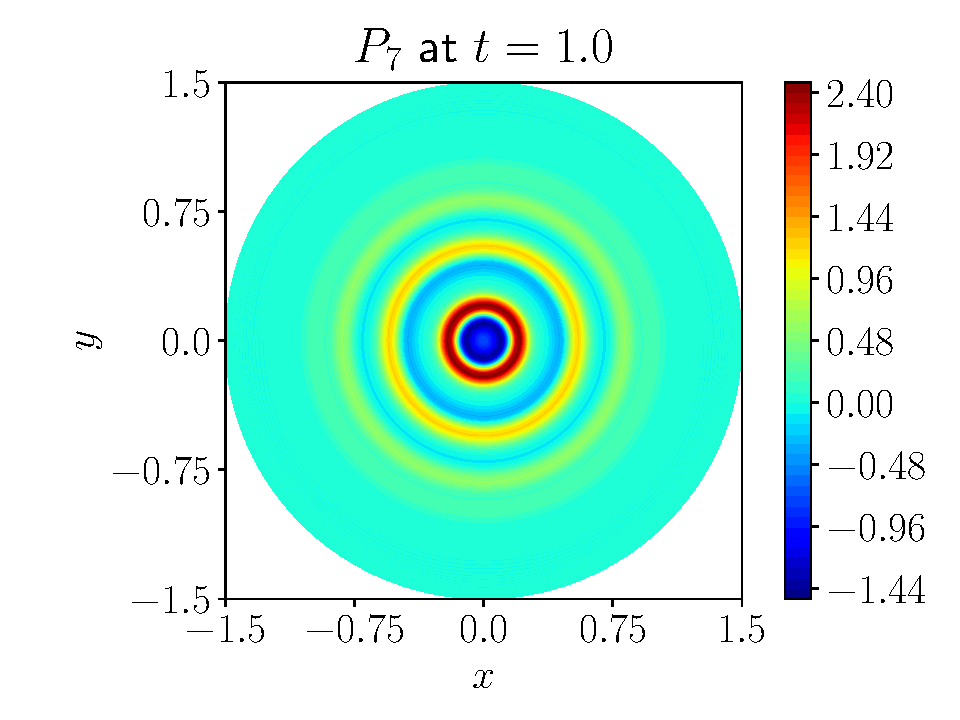
\includegraphics[height=0.4\linewidth]{figures/physical_final_p7.pdf} &
    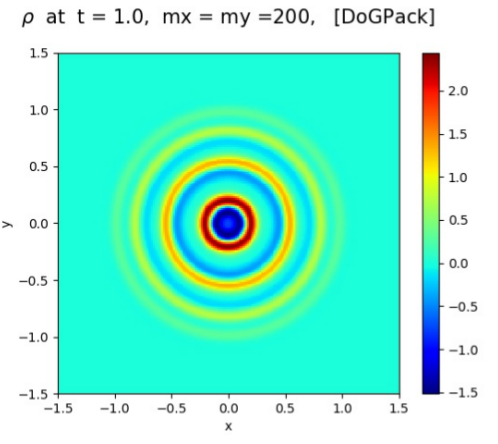
\includegraphics[height=0.4\linewidth]{figures/Minwoo_p7.png} \\
    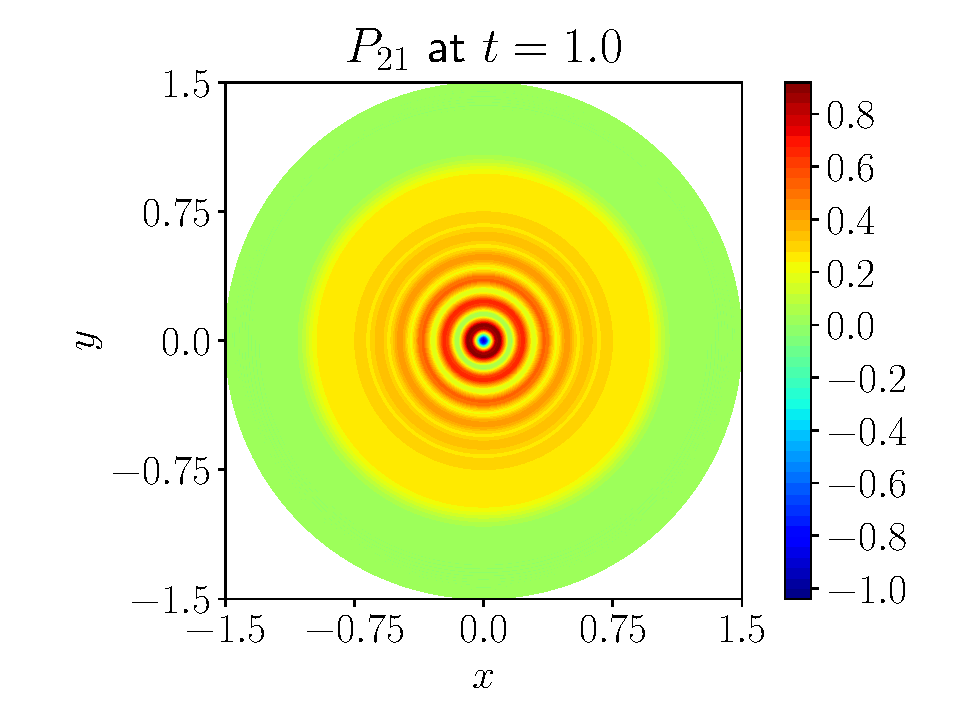
\includegraphics[height=0.4\linewidth]{figures/physical_final_p21.pdf} &
    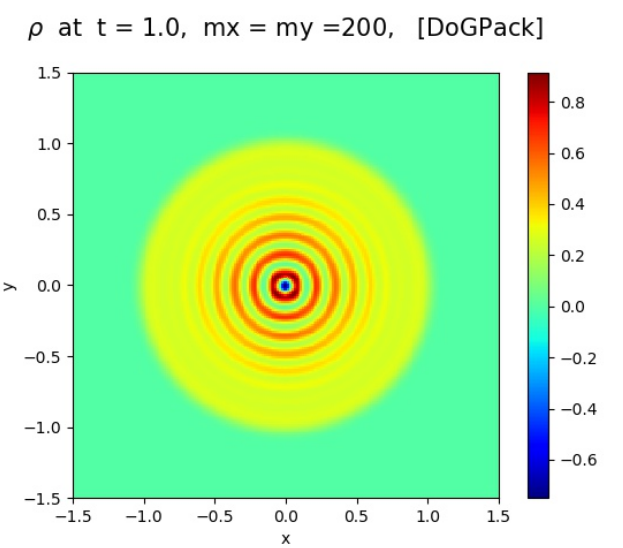
\includegraphics[height=0.4\linewidth]{figures/Minwoo_p21.png} \\
    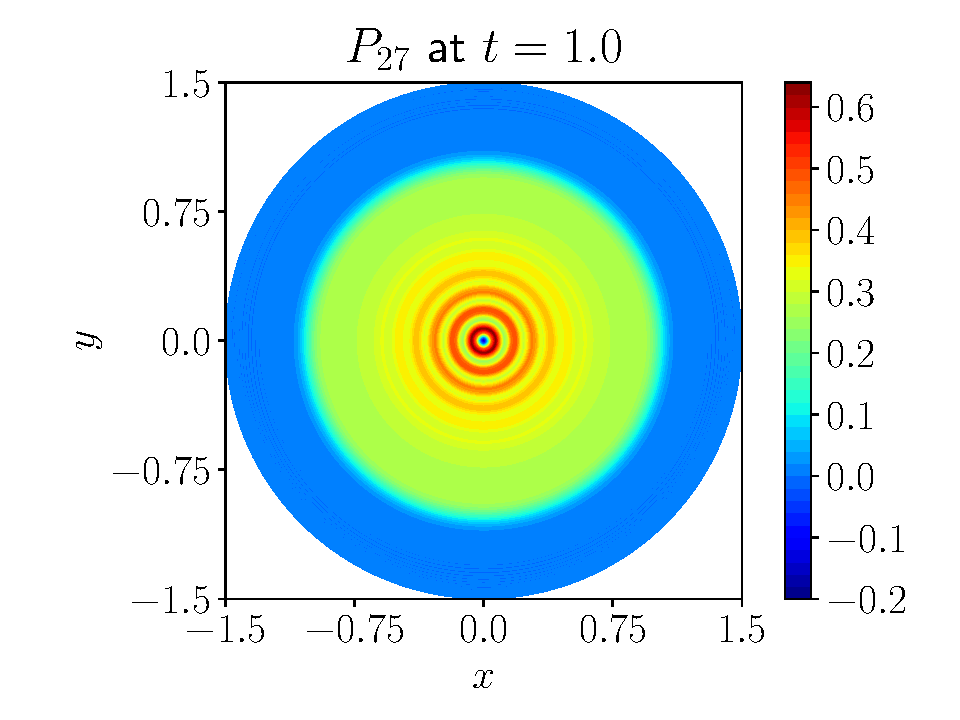
\includegraphics[height=0.4\linewidth]{figures/physical_final_p27.pdf} &
    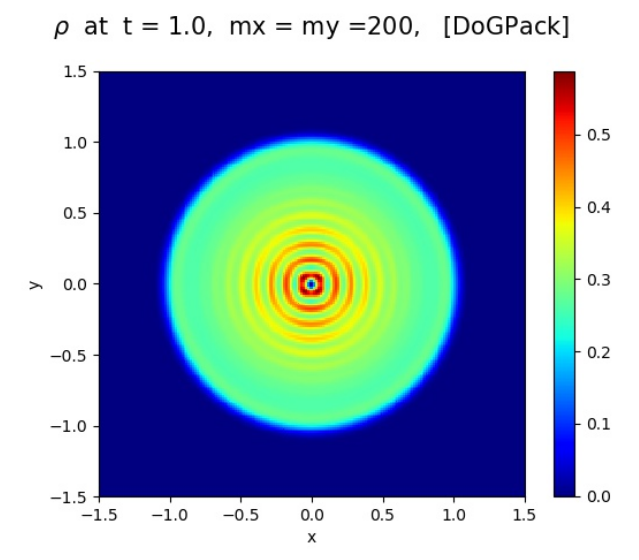
\includegraphics[height=0.4\linewidth]{figures/Minwoo_p27.png} \\
    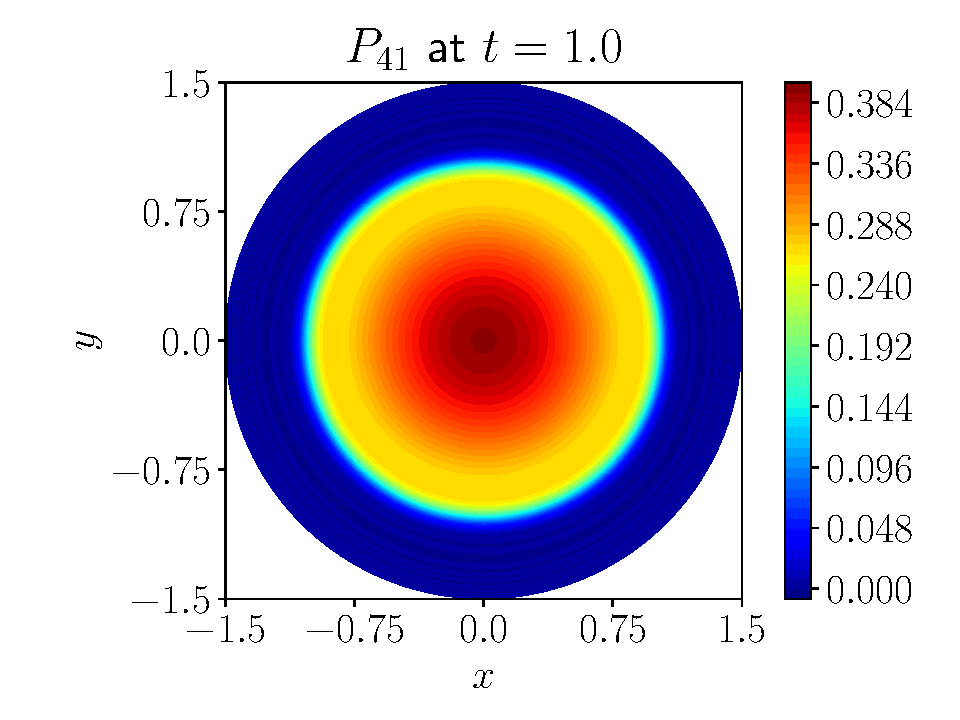
\includegraphics[height=0.4\linewidth]{figures/physical_final_p41.pdf} &
    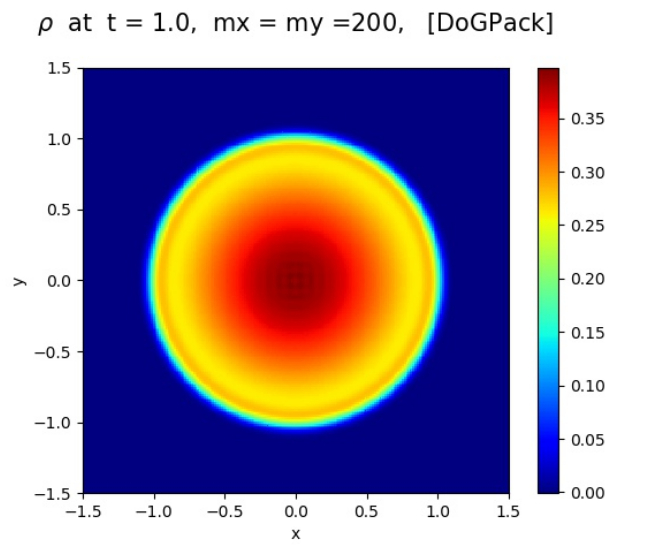
\includegraphics[height=0.4\linewidth]{figures/Minwoo_p41.png}
\end{tabular}
\end{center}    
%%%%%%%%%%%%%%%%%%%%%%%%%%%%%%%%%%%%%%%%%%%%%%%%%%%%%%%%%%%%%%%%%%
\subsection{Convergence}

In general, forming exact solutions to the $P_N$ equations is difficult.
In place of an exact solution, a high-resolution numerical solution to the radially symmetric $P_1$ equations is found with the following system of PDEs.
This formulation takes advantage of the radial symmetry to rewrite the system in polar coordinates, resulting in a 1D slice of the solution.
This PDE can be solved through any of the standard timestepping methods discussed above.
For their use as a comparison tool, this reference solution is interpolated across the 1D domain.
The solution in Radon space can then be obtained by performing a forward Radon transform of this physical solution.
\begin{align*}
	\begin{bmatrix}
		p \\
		u_{r}
	\end{bmatrix}_{, t} + 
	\begin{bmatrix}
		0 & \frac{1}{\sqrt{3}} \\
		\frac{1}{\sqrt{3}} & 0
	\end{bmatrix}
	\begin{bmatrix}
		p \\
		u_{r}
	\end{bmatrix}_{, r} = 
	\begin{bmatrix}
		-\frac{1}{\sqrt{3}} \frac{1}{r} u_{r} \\
		-\sigma u_{r}
	\end{bmatrix}
\end{align*}
To simplify the convergence studies, only a single slice of the solution obtained through the Radon method is compared.
When the $L_\infty$ norm is used, the error between the reference solution and the approximated solution is identical between any diameter of the mesh.
Thus the $L_\infty$ error across any single diameter is equal to that over the entire domain.
Additionally, radial symmetry indicates that the discretization in $\omega$ is arbitrary, and the following convergence test only takes into account the discretization across each diameter.
%\FloatBarrier
\begin{center}
    \begin{figure}[H]
        \begin{tabular}{cc}                    
            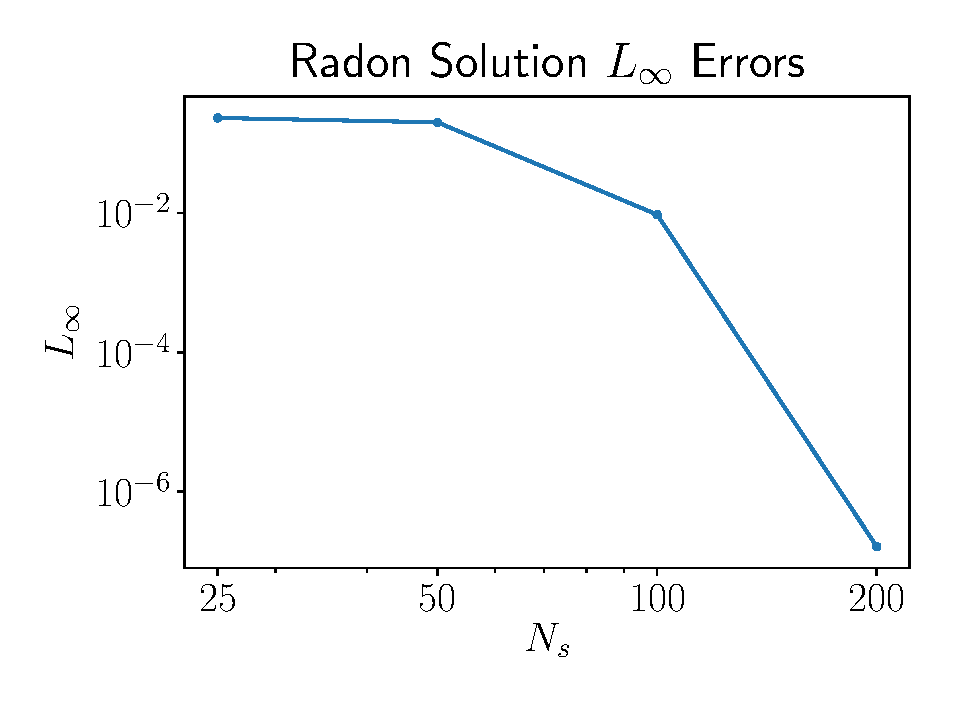
\includegraphics[height=0.35\linewidth]{figures/Convergence_Radon_Errors.pdf} &
            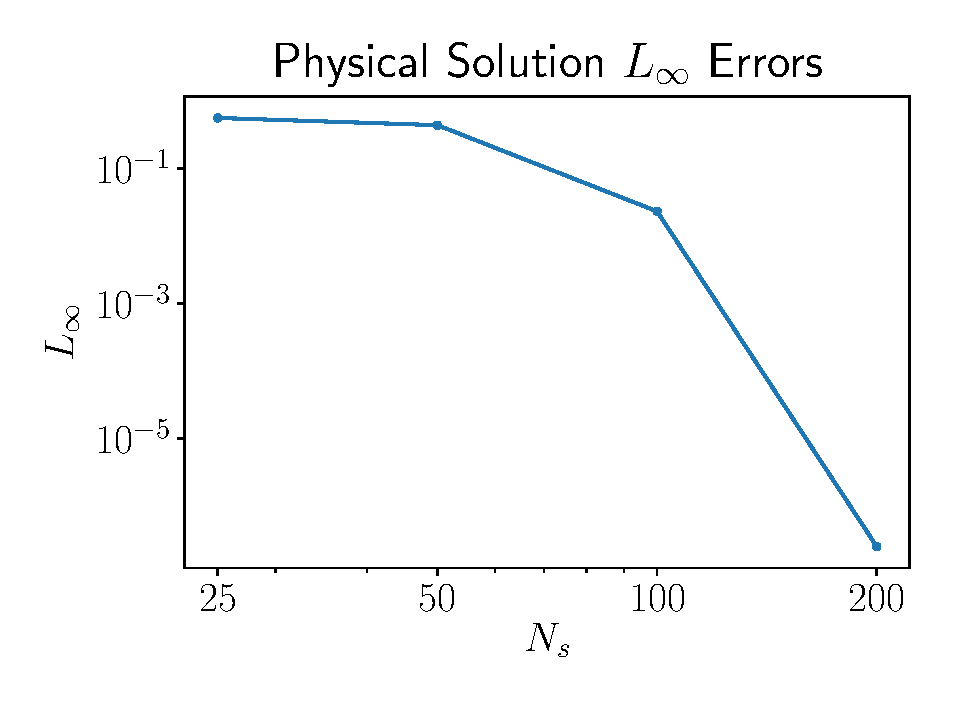
\includegraphics[height=0.35\linewidth]{figures/Convergence_Physical_Errors.pdf}
        \end{tabular}
    \captionof{figure}{$L_\infty$-Norm for radially symmetric initial conditions}
    \end{figure}
\end{center}
%\FloatBarrier
As expected, the convergence of the overall method is spectrally accurate in $N_s$.
This is because the only error present in the solution comes from insufficiently approximating the initial condition.
All other calculations, such as the interpolation, spectral differentiation, and quadrature, are all performed with spectral accuracy.

Computing convergence rates precisely is more difficult for non-radially symmetric problems, as there are no exact solutions to reference.
To counteract this, the same reference solution for the symmetric case is used, but shifted in the positive $x$ direction by some constant.
Then, the experimental $P_1$ solution can be found by translating the initial condition by the same amount, and considering the cross section across the $x$-axis.
While not a precise convergence study, one can still see that the solution approaches the true value.
For these problems, the effect of $N_s$ and $N_\omega$ must be considered independently of one another.

We begin by fixing $N_\omega = 200$, and varying $N_s$, as the timestepping is independent of the problem's symmetry.
That is to say, the solution in Radon space should be as accurate as the symmetric case.
%\FloatBarrier
\begin{center}
\begin{figure}[H]
\begin{tabular}{cc}                    
    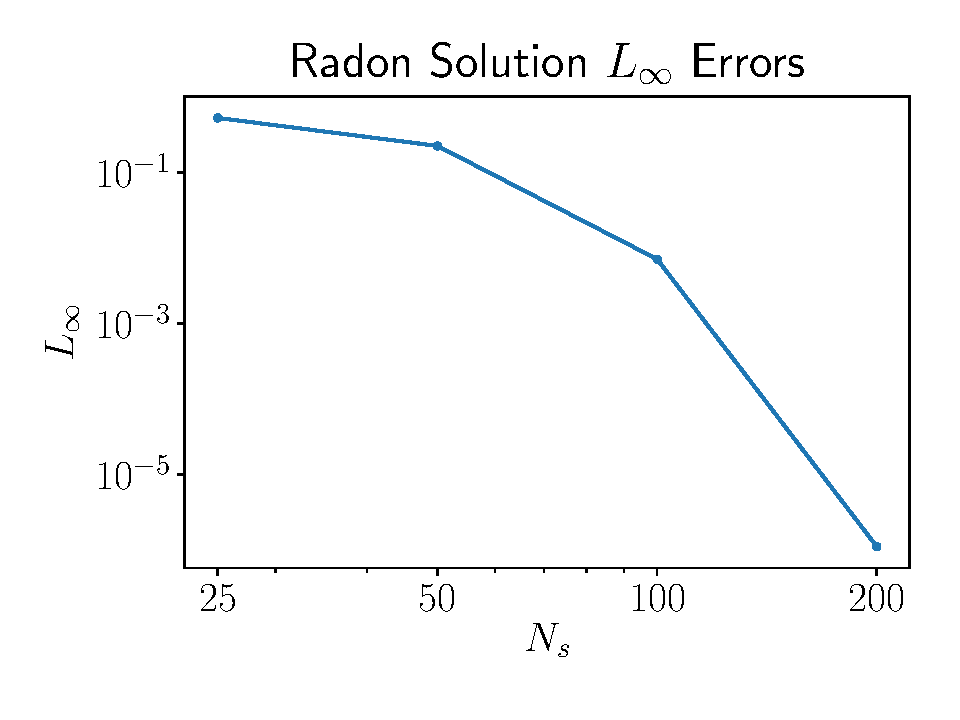
\includegraphics[height=0.35\linewidth]{figures/Convergence_Radon_Errors_Ns.pdf} &
    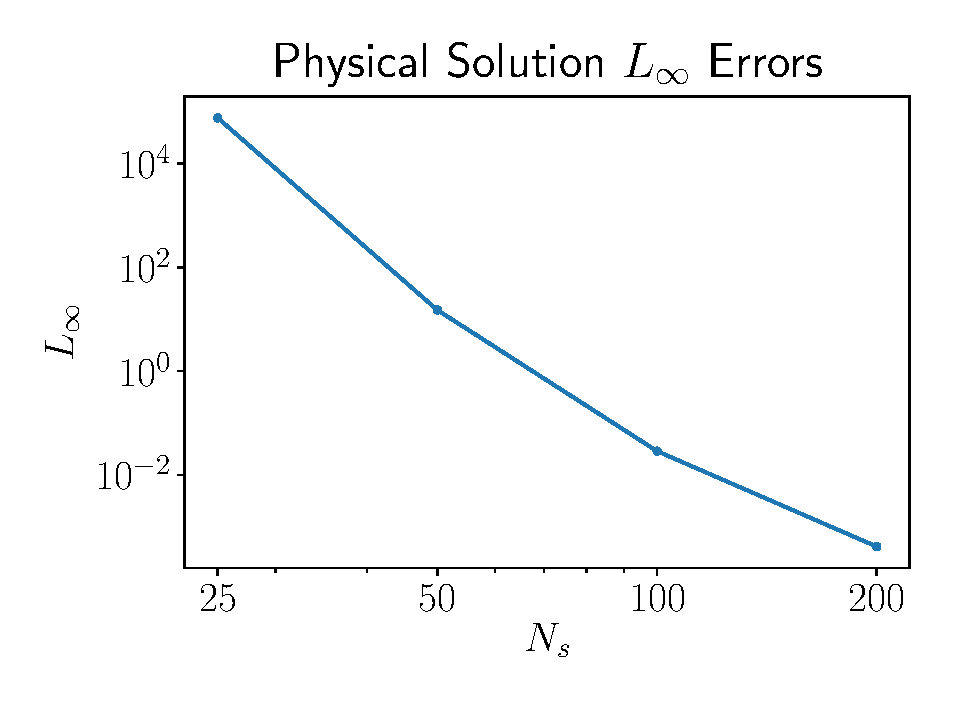
\includegraphics[height=0.35\linewidth]{figures/Convergence_Physical_Errors_Ns.pdf}
\end{tabular}
\captionof{figure}{$L_\infty$-Norm for radially symmetric initial conditions}
\end{figure}
\end{center}
%\FloatBarrier
As we see, this is the case.
We also observe that now the solution in physical space no longer has the same rate of accuracy, as the solution is limited by $N_\omega$.

We now perform the same test, but fixing $N_s$ and varying $N_\omega$.
Across each of these examples, the solution in Radon space is identical, as the timestepping is once again dependent only on the discretization along each diameter.
However, the solution in physical space is heavily dependent on the number of $N_\omega$.
We expect the solution to be fourth-order accurate, as this is the lowest convergence rate across all the component methods (owing to the radial interpolation across diameters).
%\FloatBarrier
\begin{center}
\begin{figure}[H]
	\centering
    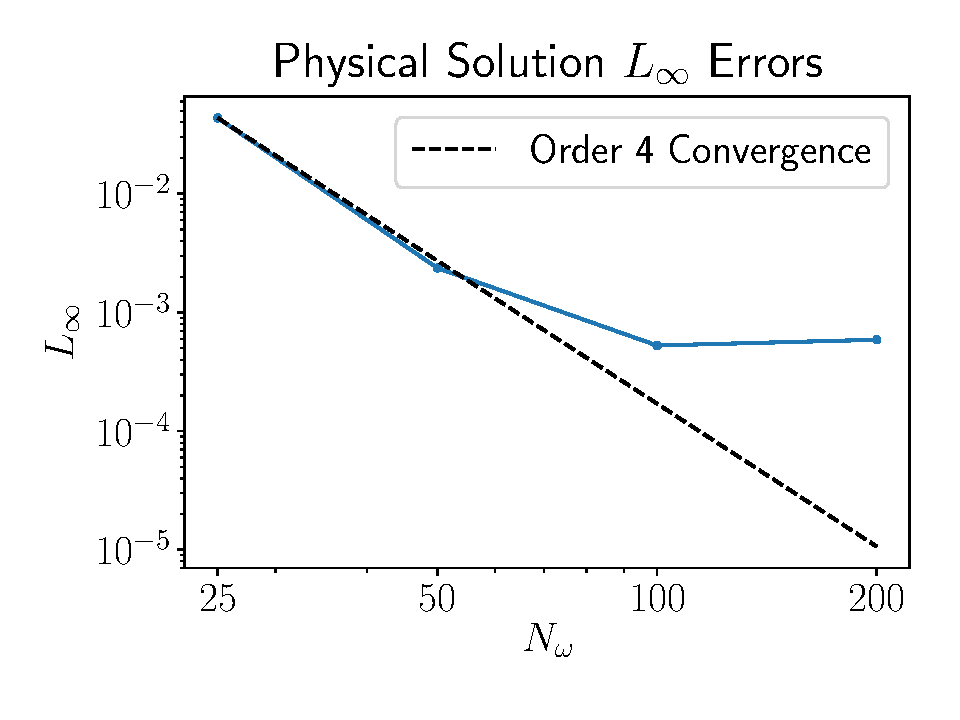
\includegraphics[height=0.35\linewidth]{figures/Convergence_Physical_Errors_Nw.pdf}
    \captionof{figure}{$L_\infty$-Norm for radially symmetric initial conditions}
\end{figure}
\end{center}
%\FloatBarrier
In practice however, we observe that while the error in the solution does decrease, it does not decrease quite as expected.
While the error is already relatively low even for low values of $N_\omega$, the desired convergence rate is only observed across the first two experiments.
Moreover the reasons for this are largely unknown at this time.
It is suspected that, rather than the method simply not being as accurate as hypothesized, there is some hidden source of error that is limiting the efficacy of the inverse Radon transform.
Possible sources of this error are a failure to accurately capture the initial condition with $N_s=200$ or a not sufficiently accurate timestepping method.
It is also possible that there is an issue with the reference solution, which is, again, only a high-resolution approximation of the true solution.
It is our hope that by addressing some or all of these issues, we can obtain results consistent with our overarching theory.
That being said, the potential payoffs of this method are great, and we hope that further investigation will illuminate this.